\documentclass[tikz,border=10pt]{standalone}
\usepackage{amsmath}
\usetikzlibrary{intersections, calc}

\begin{document}
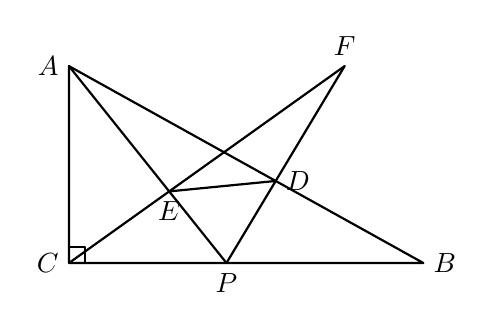
\begin{tikzpicture}[line join=round, line cap=round, >=stealth, thick]

    %% 1. 定义核心顶点坐标 (根据视觉比例设定)
    \coordinate (C) at (0,0);
    \coordinate (A) at (0,2.5);
    \coordinate (B) at (4.5,0);
    \coordinate (P) at (2,0); % P点位于CB之间

    %% 2. 绘制基础轮廓
    % 绘制直角三角形 ACB
    \draw (C) -- (B) -- (A) -- cycle;

    % 连接 AP
    \draw (A) -- (P);

    %% 3. 计算并绘制交点与延伸线
    % 定义 F 的位置（通过设定斜率或比例，图形中F在AP延长线附近，CF穿过E）
    % 为了符合原图 E, D 的位置，我们先定义辅助线
    \coordinate (F) at (3.5, 2.5);

    % 绘制线段 CF 和 PF
    \draw (C) -- (F);
    \draw (P) -- (F);

    %% 4. 自动计算交点 E 和 D
    % E 是 AP 与 CF 的交点
    \path [name path=lineAP] (A) -- (P);
    \path [name path=lineCF] (C) -- (F);
    \path [name intersections={of=lineAP and lineCF, by={E}}];

    % D 是 AB 与 PF 的交点
    \path [name path=lineAB] (A) -- (B);
    \path [name path=linePF] (P) -- (F);
    \path [name intersections={of=lineAB and linePF, by={D}}];

    % 绘制连接线段 ED
    \draw (E) -- (D);

    %% 5. 标注点名称
    % 根据位置自动偏移标签
    \node [left]  at (A) {$A$};
    \node [left]  at (C) {$C$};
    \node [below] at (P) {$P$};
    \node [right] at (B) {$B$};
    \node [above] at (F) {$F$};
    \node [below] at (E) {$E$};
    \node [right] at (D) {$D$};

    %% 6. (可选) 标注直角符号
    % 如果AC垂直BC
    \draw (0,0.2) -- (0.2,0.2) -- (0.2,0);

\end{tikzpicture}
\end{document}